\documentclass[14pt]{beamer}
\usepackage{luatexja-fontspec}
\newjfontface{\nonproportional}{BIZ UDMincho}[YokoFeatures={JFM=ujis}]
\setmainjfont[Ligatures={Common,TeX},
  ItalicFont={BIZ UDPMincho},
  ItalicFeatures={FakeSlant=0.27},
  SlantedFont={BIZ UDPMincho},
  SlantedFeatures={FakeSlant=0.18},
  BoldFont={BIZ UDPGothic Bold},
  BoldSlantedFont={BIZ UDPGothic Bold},
  BoldSlantedFeatures={FakeSlant=0.18},
  BoldItalicFont={BIZ UDPGothic Bold},
  BoldItalicFeatures={FakeSlant=0.27},
  YokoFeatures={JFM=prop}]{BIZ UDPMincho}
%\newjfontface{\nonproportional}{BIZ UDGothic}[YokoFeatures={JFM=ujis}]
\setsansjfont[Ligatures={Common,TeX},
  ItalicFont={BIZ UDPGothic},
  ItalicFeatures={FakeSlant=0.23},
  SlantedFont={BIZ UDPGothic},
  SlantedFeatures={FakeSlant=0.23},
  BoldFont={BIZ UDPGothic Bold},
  BoldSlantedFont={BIZ UDPGothic Bold},
  BoldSlantedFeatures={FakeSlant=0.23},
  BoldItalicFont={BIZ UDPGothic Bold},
  BoldItalicFeatures={FakeSlant=0.23},
  YokoFeatures={JFM=prop}]{BIZ UDPGothic}
\usepackage{beamerthemesplit}
\usepackage{caption}
\captionsetup[figure]{labelformat=empty,labelsep=none}
\usepackage{svg}
\usepackage[]{graphicx}
\graphicspath{
  {./images/}
}
\svgsetup{
  inkscapelatex=false
}

\usepackage{listings,jvlisting}
\lstset{
  language=C++,
  basicstyle=\ttfamily\footnotesize,
  % keywordstyle=\bfseries\color{green},
  showstringspaces=false,
  frame={tb},
  %numbers=left,
  xrightmargin=0\zw,
  xleftmargin=0\zw,
  % columns=[l]{fullflexible},
  columns=fixed,
  basewidth=0.5em,
  numberstyle = \footnotesize,
  frame = tbrl,
  captionpos = b,
  moredelim=[is][\color{green}\bfseries]{<\#green\#}{\#>},
  moredelim=[is][\color{blue}\bfseries]{<\#blue\#}{\#>},
  moredelim=[is][\color{red}\bfseries]{<\#red\#}{\#>},
  moredelim=[is][\color{yellow}\bfseries]{<\#yellow\#}{\#>},
  moredelim=[is][\color{magenta}\bfseries]{<\#magenta\#}{\#>},
}

\usetheme{Boadilla}
%Beamerフォント設定
\usefonttheme{professionalfonts} % Be professional!
\usepackage[T1]{fontenc}
%\usepackage{mlmodern}  % 太いComputer Modern
%\usepackage{newtxtext} % 数式以外をTXフォントで上書き
%\usepackage[deluxe,uplatex]{otf} % 日本語多ウェイト化
\renewcommand{\familydefault}{\sfdefault}  % 英文をサンセリフ体に
\renewcommand{\kanjifamilydefault}{\gtdefault}  % 日本語をゴシック体に
\usefonttheme{structurebold} % タイトル部を太字
\setbeamerfont{alerted text}{series=\bfseries} % Alertを太字
\setbeamerfont{section in toc}{series=\mdseries} % 目次は太字にしない
\setbeamerfont{frametitle}{size=\Large} % フレームタイトル文字サイズ
\setbeamerfont{title}{size=\LARGE} % タイトル文字サイズ
\setbeamerfont{date}{size=\small}  % 日付文字サイズ
%Beamer色設定
\definecolor{UniBlue}{RGB}{0,150,200}
\definecolor{AlertOrange}{RGB}{255,76,0}
\definecolor{AlmostBlack}{RGB}{38,38,38}
\setbeamercolor{normal text}{fg=AlmostBlack}  % 本文カラー
\setbeamercolor{structure}{fg=UniBlue} % 見出しカラー
\setbeamercolor{block title}{fg=UniBlue!50!black} % ブロック部分タイトルカラー
\setbeamercolor{alerted text}{fg=AlertOrange} % \alert 文字カラー
\mode<beamer>{
    \definecolor{BackGroundGray}{RGB}{254,254,254}
    \setbeamercolor{background canvas}{bg=BackGroundGray} % スライドモードのみ背景をわずかにグレーにする
}
%フラットデザイン化
\setbeamertemplate{blocks}[rounded] % Blockの影を消す
\useinnertheme{circles} % 箇条書きをシンプルに
\setbeamertemplate{navigation symbols}{} % ナビゲーションシンボルを消す
\setbeamertemplate{footline}[frame number] % フッターはスライド番号のみ

\usepackage{tikz}
\usepackage[absolute,overlay]{textpos}

\usepackage{pxrubrica} %ルビ

%教科書対応ページのマクロ
\newcommand{\textpageref}[1]{{
  \begin{textblock*}{0.4\linewidth}(285pt,5pt)
    \begin{tikzpicture}
        \node[rectangle,fill=cyan!10,text width=2.3cm, text centered,rounded corners]{教科書\\{#1}ページ};
    \end{tikzpicture}
  \end{textblock*}
}}

% 余白を広げる
\setbeamersize{text margin left=15pt, text margin right=15pt}
\setbeamertemplate{footline}[frame number]
\title{子どもIT未来塾 第6回}
\author{奥山 祐市}

\begin{document}

\frame{
   \begin{center}
    \huge{子どもIT未来塾 第6回}\\

    \vspace{34pt}
	   {\huge 音声合成と音声認識}\\
    \vspace{24pt}
    \large{奥山 祐市}\\
    \vspace{10pt}
    \large{\the\year 年 9月21日}
  \end{center}
}

\begin{frame}
	\frametitle{今日やること}
  \begin{enumerate}
    \item 音声合成
    \begin{enumerate}
      \item 音声合成とは
      \item Open JTalkとは
    \end{enumerate}
    \item 音声認識
    \begin{enumerate}
      \item 音声認識とは
      \item Juliusとは
    \end{enumerate}
  \end{enumerate}
\end{frame}

\begin{frame}
  \frametitle{音声合成}
  \vspace{30pt}
  \begin{center}
  人間の音声を人工的に作りだすこと
  \begin{figure}
    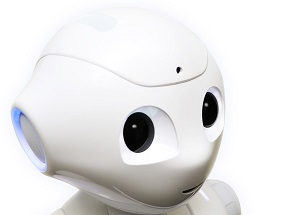
\includegraphics[width=0.5\textwidth]{chap06/text06-img001.jpg}
    \caption{Pepper (softbank)}
  \end{figure}
  \end{center}
  \textpageref{2}
\end{frame}

\begin{frame}
  \frametitle{Open JTalk}
  \begin{itemize}
    \item 音声合成のためのソフトウェア
    \item 文字(テキスト)を読み上げる
  \end{itemize}
  \begin{center}
  \includesvg[width=0.8\textwidth]{chap06/text06-img011.svg}
  \end{center}
  \textpageref{2}
\end{frame}

\begin{frame}
  \frametitle{音声認識}
  \vspace{20pt}
  \begin{itemize}
    \item 人間の声をコンピュータに認識させること
    \item 話し言葉から文字列への変換
    \item 音声の特徴を捉える
  \end{itemize}
  \begin{center}
  \begin{figure}[tbp]
  \begin{minipage}[b]{0.45\columnwidth}
    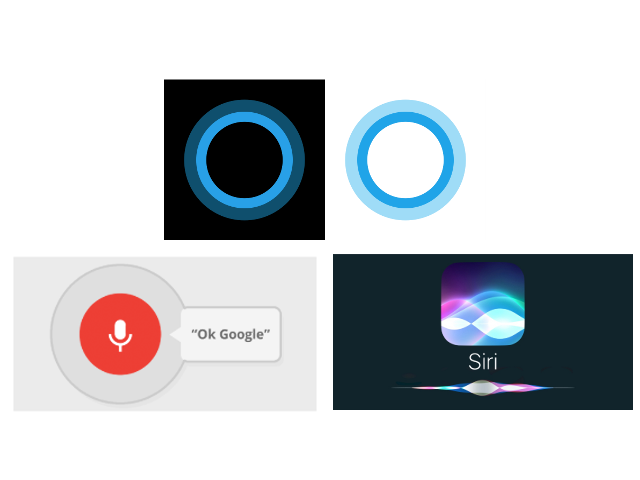
\includegraphics[width=\columnwidth]{voice_assistant.png}
    \caption{\scriptsize 携帯、スマートフォン、コンピュータの音声認識アシスタント}
  \end{minipage}
  \hspace{0.04\columnwidth}
  \begin{minipage}[b]{0.3\columnwidth}
    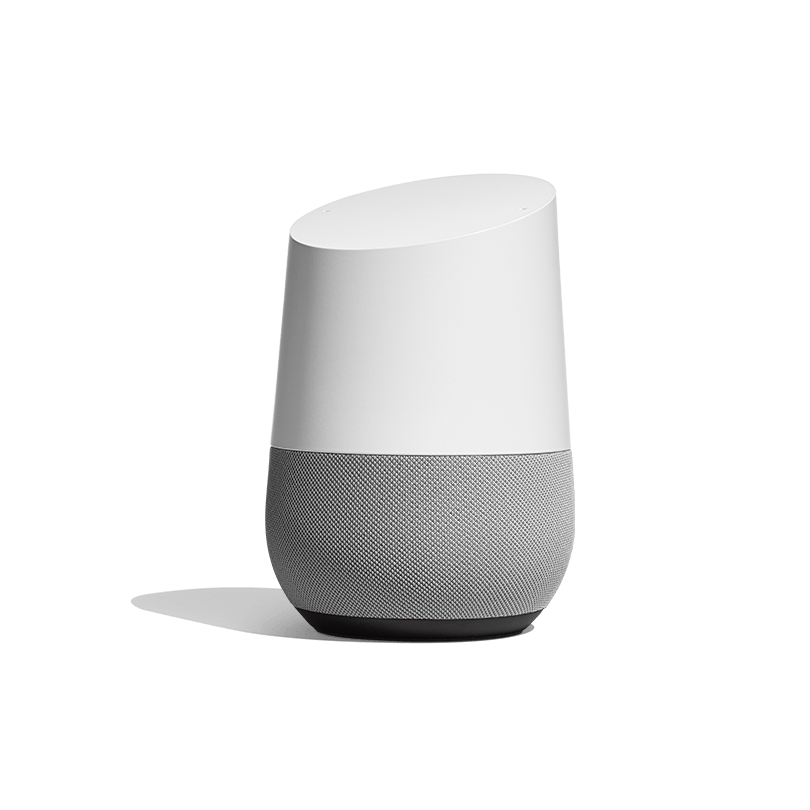
\includegraphics[width=\columnwidth]{google_home.png}
    \caption{\scriptsize Google Home}
  \end{minipage}
  \end{figure}
  \end{center}
  \textpageref{3}
\end{frame}

\begin{frame}
  \frametitle{Julius}
  \begin{itemize}
    \item 音声認識のためのソフトウェア
    \item 音声を聞き取って文字に変換する
  \end{itemize}
  \begin{center}
  \includesvg[width=0.8\textwidth]{chap06/Julius.svg}
  \end{center}
  \textpageref{3}
\end{frame}

\begin{frame}
  \begin{exampleblock}{問題を解いてみよう}
    \begin{itemize}
      \item 教科書3ページ 問題6-1(2問)
      \item 教科書3ページ 問題6-2(1問)
    \end{itemize}
  \end{exampleblock}
  \textpageref{3}
\end{frame}

\begin{frame}
  \centering
  {\Large 準備}
\end{frame}

\begin{frame}
  \frametitle{ヘッドフォンをつけよう}
  \begin{center}
  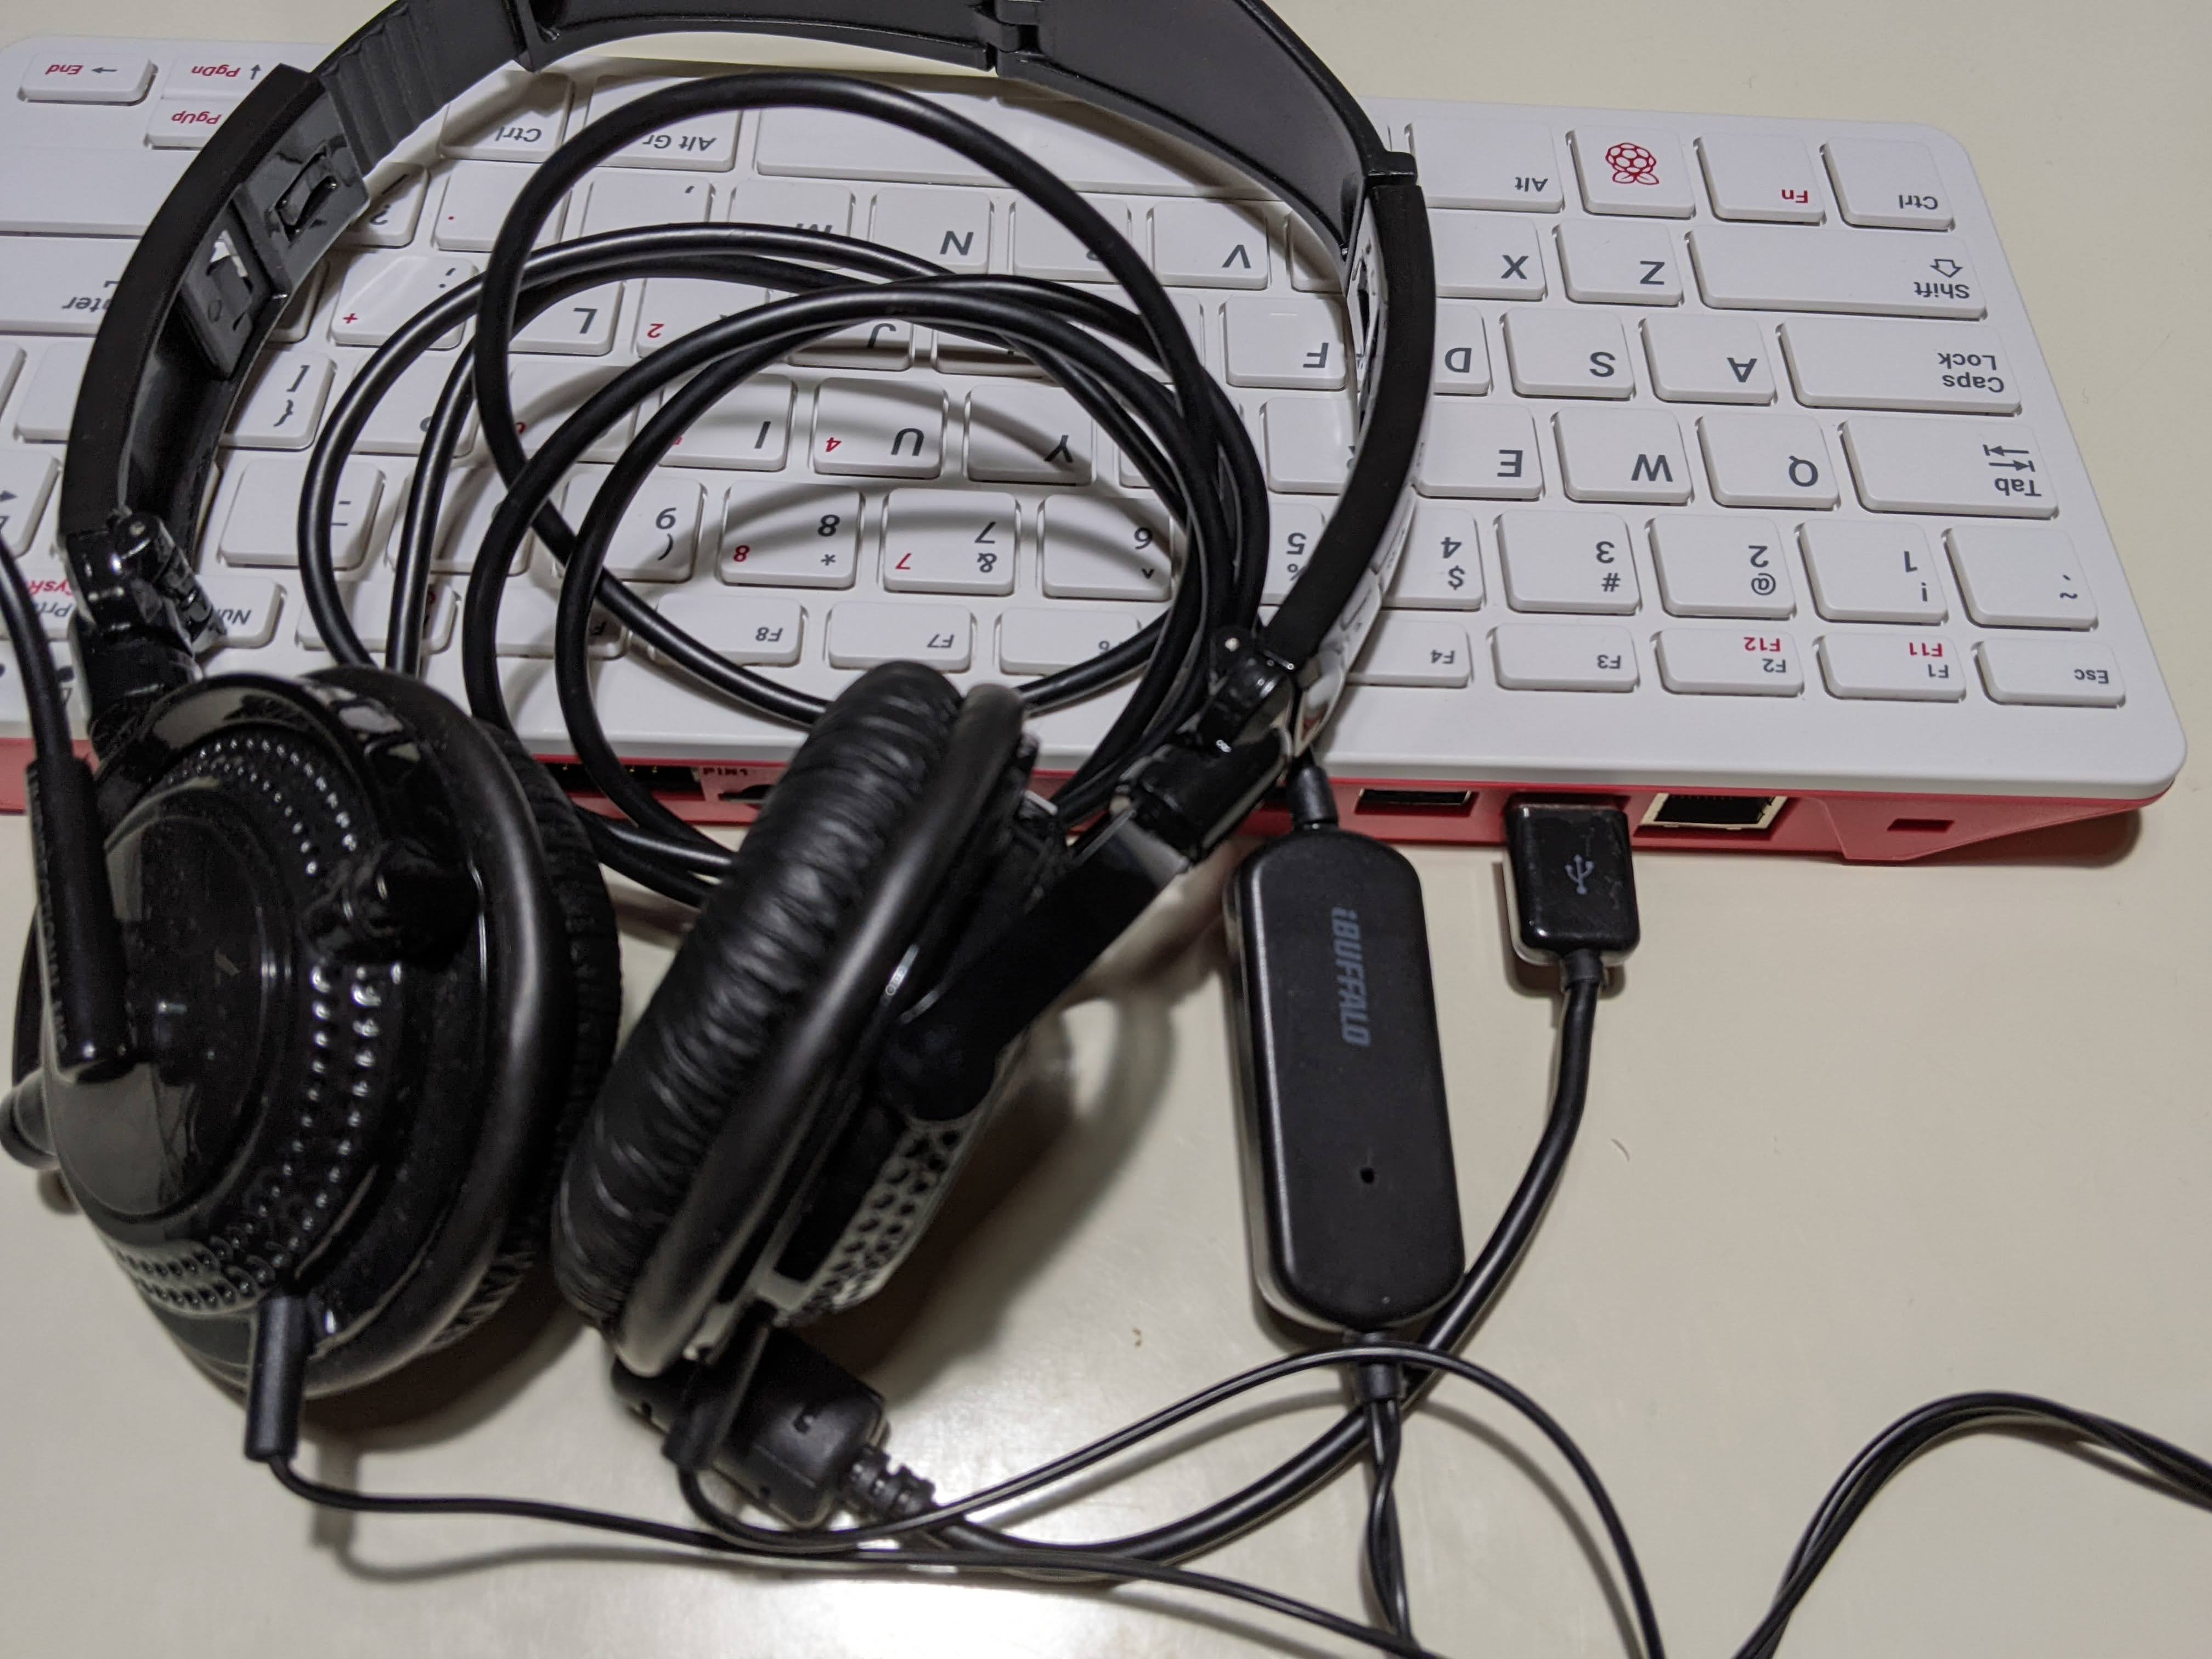
\includegraphics[width=0.8\textwidth]{how_to_connect_headset.jpg}
  \end{center}
  \textpageref{4}
\end{frame}

\begin{frame}
  \frametitle{マイクミュートについて}
  \vspace{20pt}
  \begin{itemize}
    \item ヘッドセットのコントローラに赤いランプが点いていると「マイクミュート」
    \item マイクを使うときはマイクミュートを解除しておこう
  \end{itemize}
  \begin{center}
  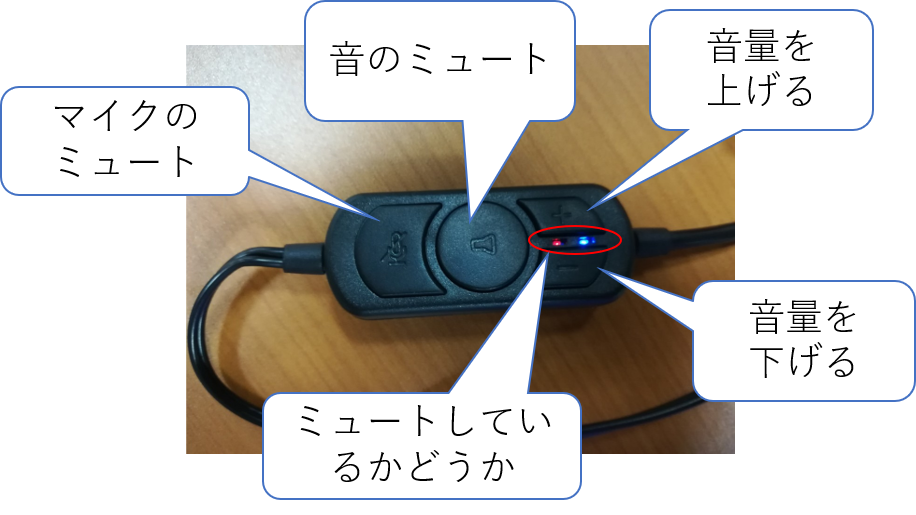
\includegraphics[width=0.8\textwidth]{chap06/text06-img004.png}
  \end{center}
  \textpageref{4}
\end{frame}

\begin{frame}
  \frametitle{マイク音量の設定}
  \begin{center}
  \begin{figure}
    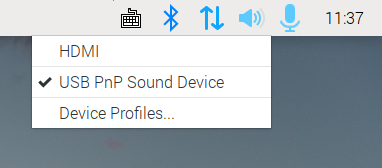
\includegraphics[width=0.5\textwidth]{select_sink.png}
    \caption{音声デバイスの選択と設定}
    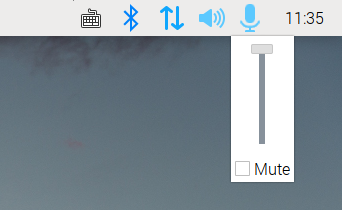
\includegraphics[width=0.5\textwidth]{microphone_volume.png}
    \caption{マイクの入力音量の調整}
  \end{figure}
  \end{center}
  \textpageref{5}
\end{frame}

\begin{frame}
  \centering
  {\Large OpenJTalk}
\end{frame}

\begin{frame}[fragile]
  \frametitle{文章を読み上げてもらう -1}
  
  \begin{lstlisting}[title=\textasciitilde/06/openjtalk.hsp,label=openjtalk.hsp]
  #include "hsp3dish.as"
  #include "jtalk.as"

  redraw 0
  mes "発話開始"
  mes "「子どもIT未来塾」"
  redraw 1
  
  <#red#jtload "子どもIT未来塾", 0	;音声ファイルを出力し、読み込む#>
  mmplay 0			<#blue#;音声ファイルを再生する#>
  stop
  \end{lstlisting}
  \textpageref{6}
\end{frame}

\begin{frame}
  \frametitle{文章を読み上げてもらう -2}
  \begin{itemize}
    \item プログラムの中の jtload "子どもIT未来塾", 0 の部分を見てみよう
    \item jtload "読ませたい文字列", <バッファ番号>
    \item ""の中の文字列を変えると、好きな言葉を読ませられるよ!
  \end{itemize}
  \textpageref{6}
\end{frame}

\begin{frame}[fragile]
  \frametitle{声音を変えてみる -1}
  \begin{lstlisting}[title=\textasciitilde/06/voice.hsp,label=voice.hsp]
  #include "hsp3dish.as"
  #include "jtalk.as"

  redraw 0
  mes "発話開始"
  mes "「子どもIT未来塾」"
  redraw 1
 
  <#red#setvoice "htsvoice-tohoku-f01/tohoku-f01-sad.htsvoice" #>
                             <#red#;音声ファイルを指定#>
  jtload "子どもIT未来塾", 0	<#blue#;音声ファイルを出力し、読み込む#>
  mmplay 0			<#blue#;音声ファイルを再生する#>
  stop
  \end{lstlisting}
  \textpageref{8}
\end{frame}

\begin{frame}
  \frametitle{声音を変えてみる -2}
  \begin{itemize}
    \item プログラムの中で音声ファイルを指定している部分を見てみよう
    \item setvoiceの右にある""の中を他のファイルに書き換えると、声音が変わるよ
    \item 他にどんな声音のファイルがあるか教科書を確認してみよう
  \end{itemize}
  \textpageref{8}
\end{frame}

\begin{frame}[fragile]
  \frametitle{読み上げる文字列に変数を使う -1}
  \begin{lstlisting}[title=\textasciitilde/06/readdate.hsp,label=readdate.hsp]
    #include "hsp3dish.as"
    #include "jtalk.as"

    <#red#date = "" + gettime(0) + "年" + 
                gettime(1) + "月" + gettime(3) + "日"#>

    redraw 0
    mes "日付を読み上げます"
    mes date
    redraw 1

    jtload date, 0 <#blue#;date変数に代入されている文字を
                          音声ファイルにし、読み込む#>
    mmplay 0 <#blue#;音声ファイルを再生する#>
    stop
  \end{lstlisting}
  \textpageref{10}
\end{frame}

\begin{frame}
  \frametitle{読み上げる文字列に変数を使う -2}
  \begin{itemize}
    \item openjtalk は date 変数に代入された文字列を読む
    \item gettime 関数で今日の日付を取得する
    \begin{itemize}
       \item 0 = 年、1 = 月、2 = 曜日、3 = 日
       \item 4 = 時間、5 = 分、6 = 秒、7 = ミリ秒
    \end{itemize}
    \item gettime関数の()の中を変えると、時間や曜日も読ませられるよ!
  \end{itemize}
  \textpageref{10}
\end{frame}

\begin{frame}[fragile]
  \frametitle{読み上げる文字列に変数を使う -3}
  \begin{lstlisting}[title=\textasciitilde/06/readcalc.hsp,label=readcalc.hsp]
    #include "hsp3dish.as"
    #include "jtalk.as"

    a = 3
    b = 2

    <#blue#;問題描画#>
    redraw 0
    mes = "" + a + " + " + b
    redraw 1

    <#blue#;問題読み上げ#>
    jtload "" + a + "たす" + b, 0
    mmplay 0
    <#red#wait 100#>
  \end{lstlisting}
  \textpageref{12}
\end{frame}

\begin{frame}[fragile]
  \frametitle{読み上げる文字列に変数を使う\\(コード続き)}
  \begin{lstlisting}[title=\textasciitilde/06/readcalc.hsp,label=readcalc.hsp]
    <#blue#;答え計算#>
    kotae = a + b

    <#red#;答え読み上げ
    jtload "こたえは" + kotae, 1
    mmplay 1#>

    <#blue#;答え描画#>
    redraw 0
    mes "" + a + " + " + b
    mes "= " + kotae
    redraw 1

    wait 30
    stop
  \end{lstlisting}
  \textpageref{12}
\end{frame}

\begin{frame}
  \frametitle{読み上げる文字列に変数を使う(4)}
  \begin{itemize}
    \item a + b の計算結果を kotae に代入
    \item openjtalk はkotaeに代入された値を読んでいる
    \item 問題と答えを読む音声が重ならないように wait 100 で少し待っている
  \end{itemize}
  \textpageref{12}
\end{frame}

\begin{frame}
  \begin{exampleblock}{問題を解いてみよう}
    \begin{itemize}
      \item 教科書7ページ 問題6-3(2問)(1問は宿題)
      \item 教科書9ページ 問題6-4(2問)(1問は宿題)
      \item 教科書11ページ 問題6-5(2問)(1問は宿題)
      \item 教科書13ページ 問題6-6(2問)(1問は宿題)
    \end{itemize}
\end{exampleblock}
  \textpageref{7,9,11,13}
\end{frame}

\begin{frame}
  \centering
  {\Large Julius}
\end{frame}

\begin{frame}
  \frametitle{Juliusを使ってみる(1)}
  \begin{itemize}
    \item run-linux-gmm.sh
    \item \<\<please speak\>\>がでるまで待つ
  \end{itemize}
  \begin{center}
  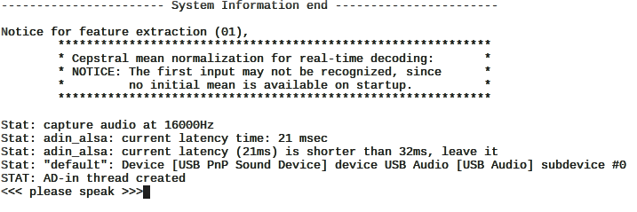
\includegraphics[width=0.8\textwidth]{chap06/text06-img009.png}
  \end{center}
  \textpageref{14}
\end{frame}

\begin{frame}
  \begin{exampleblock}{問題を解いてみよう}
    \begin{itemize}
      \item 教科書14ページ 問題6-7(1問)
    \end{itemize}
\end{exampleblock}
  \textpageref{14}
\end{frame}

\begin{frame}
  \frametitle{Juliusを使ってみる(2)}
  \begin{itemize}
    \item 果物の名前を話かけてみよう
    \begin{center}
      {\small りんご みかん ぶどう もも あけび あんず いちご\\いちじく かき スイカ すもも 	なし メロン}
    \end{center}
    \item コンピュータは正しく言葉を認識してくれたかな?
    \item 話しかけた単語とターミナルに出てくる単語が同じか友達と話合ってみよう
  \end{itemize}
  \textpageref{14}
\end{frame}

\begin{frame}
  \frametitle{単語辞書}
  \begin{itemize}
    \item すべての言葉をコンピュータに理解してもらうのは大変
    \item そのままのJuliusでは限界がある
    \item コンピュータに理解してほしい言葉をまとめた辞書を作ると改善される!
  \end{itemize}
  \textpageref{15}
\end{frame}

\begin{frame}
  \frametitle{単語辞書を使ってみる}
  \begin{itemize}
    \item 単語辞書を使ってJuliusをためす
    \begin{itemize}
      \item julius.sh kudamono.dic
      \item 以下の単語が登録されているよ。マイクに話しかけてみよう
    \end{itemize}
  \end{itemize}
  \begin{center}
    {\small りんご みかん ぶどう もも あけび あんず いちご いちじく かき スイカ すもも 	なし メロン}
  \end{center}
  \textpageref{15}
\end{frame}

\begin{frame}
  \begin{exampleblock}{問題を解いてみよう}
    \begin{itemize}
      \item 教科書15ページ 問題6-8(2問)
    \end{itemize}
\end{exampleblock}
  \textpageref{15}
\end{frame}

\begin{frame}
\frametitle{結果を見てみよう} 
  \begin{center}
  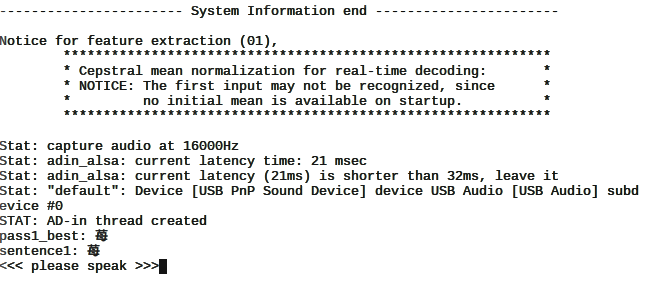
\includegraphics[width=0.8\textwidth]{julius_demo_strawberry.png} \\
  \end{center}
  話かけた単語とターミナルに表示される単語は一致しているかな?
  \textpageref{15}
\end{frame}

\begin{frame}
  \frametitle{単語辞書を作ってみよう -1}
  \begin{itemize}
    \item 認識させたい単語を登録しよう
    \begin{itemize}
      \item kudamono.yomiを参考に…
      \item \<コンピュータが使う名前\> \<読み方\>
      \renewcommand{\theenumi}{\roman{enumi}}
      \begin{enumerate}
        \item りんご
        \item ぶどう
        \item みかん
      \end{enumerate}
    \end{itemize}
    \item \<コンピュータが使う名前\>には日本語も使えるよ
    \begin{itemize}
      \item 林檎 りんご
      \item ブドウ ぶどう
      \item みかん みかん
    \end{itemize}
  \end{itemize}
  \textpageref{16}
\end{frame}

\begin{frame}
  \frametitle{単語辞書を作ってみよう -2}
  \begin{itemize}
    \item mousepadで自分だけの辞書を作ってみよう
    \begin{itemize}
      \item mousepad jisho.yomi
    \end{itemize}
    \item 例えば…
    \begin{itemize}
      \item 家電辞書
      \item 動物辞書
      \item 植物辞書
    \end{itemize}
  \end{itemize}
  \textpageref{16}
\end{frame}

\begin{frame}
  \frametitle{単語辞書を作ってみよう -3}
  \begin{itemize}
    \item .yomi : テキストファイル
    \item .dic : コンピュータが読めるファイル
    \begin{itemize}
      \item yomiはコンピュータが読めないので変換する必要がある
    \end{itemize}
  \end{itemize}
  \textpageref{3}
\end{frame}

\begin{frame}
  \frametitle{単語辞書を作ってみよう -4}
  \begin{itemize}
    \item convert\_yomi.sh コマンド
    \begin{itemize}   
      \item コンピュータ用の辞書へと変換してみよう
      \item convert\_yomi.sh jisyo.yomi  jisyo.dic
    \end{itemize}
    \item julius.sh コマンド
    \begin{itemize}
      \item 自分の作った辞書で音声認識をしてみよう
      \item julius.sh jisyo.dic
    \end{itemize}
    \item コンピュータは上手く言葉を理解してくれるかな?
  \end{itemize}
  \textpageref{16}
\end{frame}

\begin{frame}
  \begin{exampleblock}{問題を解いてみよう}
    \begin{itemize}
      \item 教科書17ページ 問題6-9(5問)(1問は宿題)
    \end{itemize}
  \end{exampleblock}
  \textpageref{17}
\end{frame}

\begin{frame}
  \frametitle{HSPでJuliusの認識結果を使う -1}
  \begin{figure}
    \includesvg[width=\linewidth]{images/chap06/JuliuswithHSP.svg}
  \end{figure}
  \textpageref{18}
\end{frame}

\begin{frame}[fragile]
  \frametitle{HSPでJuliusの認識結果を使う -2}
  \begin{lstlisting}[title=\textasciitilde/06/julius.hsp,label=julius.hsp]
  #include "hsp3dish.as"
  #include "julius.as"

  redraw 0
  pos 0, 0
  mes "Loading Julius..."
  redraw 1

  init_julius "kudamono.dic" <#blue#;辞書ファイル読み込み#>

  sockidx = 0
  domain = "127.0.0.1"
  PORT = 10500
  \end{lstlisting}
  \textpageref{19}
\end{frame}

\begin{frame}[fragile]
  \frametitle{HSPでJuliusの認識結果を使う -3}
  \begin{lstlisting}[title=\textasciitilde/06/julius.hsp,label=julius.hsp]
  sockopen sockidx, domain, PORT

  if stat != 0 { <#blue#;エラー処理#>
  *errorjulius
    redraw 0
    pos 0, 0
    mes "Error in opening socket"
    redraw 1
    await 30
    goto *errorjulius
    stop
  }

  sdim words, 4096, 0
  ddim cm, 0
  \end{lstlisting}
  \textpageref{19}
\end{frame}

\begin{frame}[fragile]
  \frametitle{HSPでJuliusの認識結果を使う -4}
  \begin{lstlisting}[title=\textasciitilde/06/julius.hsp,label=julius.hsp,basicstyle=\scriptsize]
  repeat -1
    if is_recieved(sockidx) = 0 {
      get_word_list words, cm
      len =  "L1 " + length(words)
      repeat length(words)
        if cm(cnt) > 0.5 { <#blue#;単語信頼度が0.5より大きいとき#>
            ans =  "" + cnt + ": " + words(cnt) + " CM = " + cm(cnt)
        } <#blue#;words(cnt)が認識された文字、cm(cnt)が単語信頼度#>
      loop
    }
    redraw 0
    pos 0,0
    mes len
    mes ans
    redraw 1
    await 30
  loop
  \end{lstlisting}
  \textpageref{19}
\end{frame}

\begin{frame}
  \begin{exampleblock}{問題を解いてみよう}
    \begin{itemize}
      \item 教科書20ページ 問題6-10(2問)
    \end{itemize}
  \end{exampleblock}
  \textpageref{20}
\end{frame}

\begin{frame}[fragile]
  \frametitle{音声でLEDのON OFFをする -1}
  \begin{lstlisting}[title=\textasciitilde/06/ledvoice.hsp,label=ledvoice.hsp]
    #include "hsp3dish.as"
    #include "julius.as"

    redraw 0
    pos 0, 0
    mes "Loading Julius..."
    redraw 1

    init_julius " \textasciitilde /06/onoff.dic" <#blue#;辞書を読み込む#>

    sockidx = 0
    domain = "127.0.0.1"
    PORT = 10500
  \end{lstlisting}
  \textpageref{22}
\end{frame}

\begin{frame}[fragile]
  \frametitle{音声でLEDのON OFFをする -2}
  \begin{lstlisting}[title=\textasciitilde/06/ledvoice.hsp,label=ledvoice.hsp]
    if stat != 0 {
      redraw 0
      mes "Error in opening socket"
      redraw 1
      wait 30
      stop
    }

    sdim wrods, 4096, 0
    ddim cm, 0
  \end{lstlisting}
  \textpageref{22}
\end{frame}

\begin{frame}[fragile]
  \frametitle{音声でLEDのON OFFをする -3}
  \begin{lstlisting}[title=\textasciitilde/06/ledvoice.hsp,label=ledvoice.hsp,basicstyle=\scriptsize]
    repeat -1
    if is_recieved(sockidx) = 0 {
      get_word_list words, cm
      repeat length(words)
        if cm(cnt) > 0.7 {                <#blue#;単語信頼度が0.7より大きいとき#>
          if words(cnt) = "ON" {          <#blue#;認識された文字がONのとき#>
            gpio 17, 1                    <#blue#;GPIO17のLEDを光らせる#>
          }else : if words(cnt) = "OFF" { <#blue#;認識された文字がOFFのとき#>
            gpio 17, 0                    <#blue#;GPIO17のLEDを消す#>
          }
        }
      loop
    }
    redraw 0
    pos 0,0
    mes "話しかけてLEDのONとOFFをしよう"
    redraw 1
    await 30
  \end{lstlisting}
  \textpageref{22}
\end{frame}

\begin{frame}
  \begin{exampleblock}{問題を解いてみよう}
    \begin{itemize}
      \item 教科書23ページ 問題6-11(5問)(2問は宿題)
    \end{itemize}
  \end{exampleblock}
  \textpageref{23}
\end{frame}

\begin{frame}
  \frametitle{宿題}
  \begin{itemize}
    \item 教科書24ページ
    \begin{itemize}
      \item 5問の内、1問だけ挑戦しよう
      \item レベルアップしたい人は、5問全部に挑戦してみよう
    \end{itemize}
  \end{itemize}
  \textpageref{24}
\end{frame}

\begin{frame}
  \frametitle{数を認識させてみよう(発展)}
  \begin{itemize}
    \item 数を認識できる
    \begin{itemize}
      \item いち、じゅうさん、せんよんひゃくさんじゅうなな、など
    \end{itemize}
    \item 数を認識させるには「文法」を使う
    \begin{itemize}
      \item 1000(千)まで認識させたかったら1000個以上の単語を登録
      \begin{itemize}
        \item 1(いち)から1000(千)まで登録
        \item 同じ数字でも違う読み(7:なな、しち)
      \end{itemize}
      \item 文法でルールを決める
    \end{itemize}
    \item 参考:
    \begin{itemize}
      \item http://www.atmarkit.co.jp/fxml/ddd/ddd004/ddd004-bnf.html
      \item http://julius.osdn.jp/index.php?q=doc/grammar.html
    \end{itemize}
  \end{itemize}
\end{frame}

\begin{frame}
  \centering
  実験
\end{frame}

\begin{frame}
  \frametitle{OpenJTalkやJuliusでできることを考えよう}
  \begin{itemize}
    \item 例えば…
    \begin{itemize}
      \item ボタンを押すと話してくれる
      \item 気温や湿度を教えてくれる
      \item 指示した色のLEDを光らせてくれる
      \item 時刻を聞くと時刻を話してくれる
      \item 日付を聞くと日付を話してくれる
    \end{itemize}
    \item 例を参考に何が作れるかを自分で考えてみよう
  \end{itemize}
\end{frame}

\begin{frame}
  \frametitle{作りたいものを考えよう}
  \begin{itemize}
    \item OpenJTalkやJuliusを使って作りたいものを考えてみよう(5-10分)
    \item チームのみんなで作りたいものを発表してみよう、一緒に考えてみよう(5-10分)
    \begin{itemize}
      \item むずかしさはどれくらいだろう
      \item どうやって作ればいいだろう
    \end{itemize}
  \end{itemize}
\end{frame}
\begin{frame}
  \frametitle{手順}
  \begin{enumerate}
    \item 演習用のフォルダを作る
    \item 必要なファイルをフォルダにコピーしよう
    \begin{itemize}
      \item hspファイル
      \item yomiファイル
      \item htsvoiceファイル
    \end{itemize}
    \item プログラミングをしてみよう
    \begin{itemize}
      \item hspファイルを書き換えてみる
      \item 新しくhspファイルを作ってみる
    \end{itemize}
  \end{enumerate}
\end{frame}

\begin{frame}
  \frametitle{できたものをチームのみんなに教えよう}
  \begin{itemize}
    \item どんなものを作ったか
    \item 工夫したところはどこか
    \item どうしてその作品を作ったか
  \end{itemize}
  実際に作品を動かしてみんなに見せてみよう!
\end{frame}

\end{document}
